\chapter{Model specifications} \label{ch:model_specs}

This chapter presents the physical aspects of the model used throughout the report. The model has four main parts, namely the environment, the snake robot, the obstacles and the desired path. The goal of the snake robot is at all times to interact with the obstacles close to the path and use them to propel itself forward along the path. The value of all variables needed to express the model and problem are assumed known at all times.

\section{Assumptions}

Some of the following assumptions are taken from \cite{StavdahlNote} and \cite{liljeback2010hybrid}, whilst assumption 10-11 are specific for this project.

\begin{enumerate}
    \item All parts of the model are assumed to be rigid
    \item The robot has $n$ joints and all links have length $l$ and mass $m$.
    \item We consider only flat, 2-dimensional cases.
    \item The robot has no lateral extension.
    \item There is no friction. 
    \item Obstacles have of no spatial extent, only a static position in the plane.
    \item There exists a predetermined desired continuous path $S$.
    \item The robot is considered to be "on the path" whenever all joint centers coincide with the path.
    \item The robot is initially on or close to the path.
    \item Any link is in contact with at most one obstacle at the time.
    \item All energy from a link colliding with another link is dissipated.
    \item During an impact with an obstacle, the configuration of the snake robot, $\mathbf{q}$, remains unaltered while the velocity, $\mathbf{\dot{q}}$, will generally experience a jump.
\end{enumerate}

%----------------------------------------------------------------------------------
%----------------------------------------------------------------------------------

\section{Further model description}

\subsection{The snake robot}
The snake robot itself is modeled as a simple planar robot manipulator with links and joints. The main difference between the snake robot and a classic robot manipulator is the property that the snake robot is not physically attached to any fixed point in the world. This frees one constraint. However, it is still relevant to express the position of the last link of the snake, also denoted as the tail. This is performed by introducing two virtual joints to the model; one translational and one rotational attached to the base frame. These joints are not controllable and merely for describing the kinematics, dynamics and constraints. The model of the snake robot is visualized in figure \ref{fig:2_kin}. Real robot links are blue, and the virtual ones are green.

\begin{figure}
    \centering
    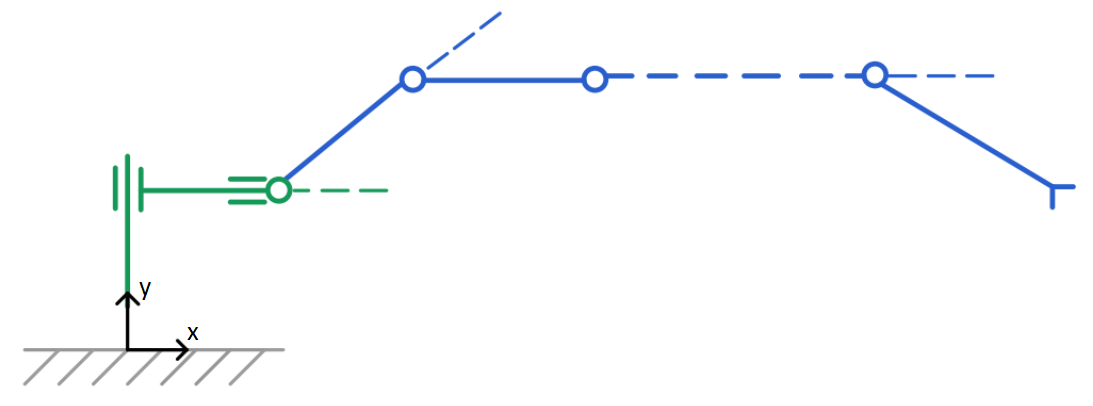
\includegraphics[width=0.9\textwidth]{figures/kinematics_noname.PNG}
    \caption{Model of snake robot with $n$ links}
    \label{fig:2_kin}
\end{figure}

%----------------------------------------------------------------------------------
%----------------------------------------------------------------------------------

\subsection{The environment}
The environment is the (x,y)-plane in figure \ref{fig:2_kin}.

%----------------------------------------------------------------------------------
%----------------------------------------------------------------------------------


\subsection{The obstacles}

The obstacles are modeled as rigid points in the plane. However, as a consequence of the discrete nature of the simulator, there is a "safety barrier" around every obstacle defining the area in which contact is present. This contact is still modeled as a point contact. The barriers can be seen as the red circles in figure \ref{fig:2_kin_obst}. The points the circles are surrounding are the actual obstacles.

\begin{figure}
    \centering
    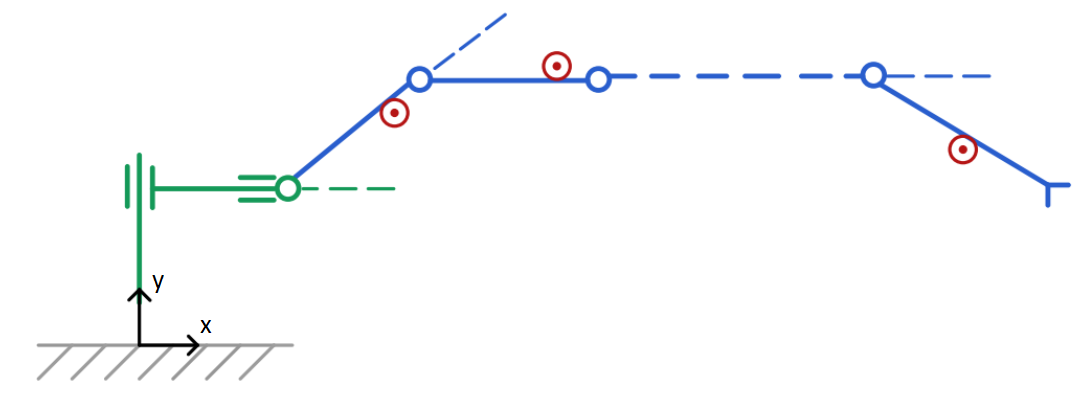
\includegraphics[width=0.9\textwidth]{figures/kinematics_obstacles_noname.PNG}
    \caption{Model of snake robot and obstacles}
    \label{fig:2_kin_obst}
\end{figure}

%----------------------------------------------------------------------------------
%----------------------------------------------------------------------------------

\subsection{The optimal path}

The path is in this report made out of straight lines and quadrants with radius equal to two times the link length $l$. There is no gap between these segments, following from the assumption of a continuous path.